
\subsubsection*{Rate of Decay}
\label{sec:findings-expts-decay}

%%%
In addition to the learning rate,
the decay parameter $d$ was also adjusted to see what sort of effect it
would have on learning.
%
Instead of the default decay rate of 10\%,
rates ranging from 0\% to 50\%
were tested to demonstrate the effect of temporal difference learning.
%%%

\paragraph*{Results}

%%%
% TODO: verify results after rerun
%%%

%%%
As can be seen in Figure~\ref{fig:expts-decay-comp},
the decay rate had no effect on the behavioral trends learned.\footnote{
	At the time of this draft,
	this is pure speculation as the actual experiment ran with a bug and needs
	to be re-run for now.
	% TODO: remove footnote and ensure accuracy of stated conclusions
}
%
However,
as expected,
the rate of learning of these behaviors in earlier states is most affected
by this parameter.
%
With lower decay rates,
more of the responsibility for the final result of the game is transferred
to earlier game states.
%
It is worthwhile to note just how clearly
the sinusoidal wave along the diagonal takes form
and subsequently loses amplitude
when there is no decay.
%
While this would seemingly indicate that earlier states needed to be
% TODO: ^^^ finish this thought
%
Contrarily,
with higher decay rates,
it is nearly impossible to learn earlier game states,
so behavior remains random,
as clearly seen when $d = 0.50$.
%
For explanation,
a typical cribbage game will take approximately ten hands
to complete.
%
At this rate,
the first states will be adjusted by a factor of
$(1-d)^{10} = (0.5)^{10} \approx 0.00098$.
%
Even over the course of one million games,
this small magnitude of modification,
combined with the rate of visitation of a single state,
is not enough for any meaningful learning to occur.
% TODO: ^^^ make sure accurate when real results happen
%%%

% fig:expts-decay-comp
\begin{figure}[h]
	\centering

	\begin{tabular}{c | l l l l}
		% Outline:
		%   s\g |  250k | 500k | 750k | 1mm
		%   0.00
		%   0.10
		%   0.25
		%   0.50
		$d$ \textbf{\textbackslash} game & 250,000 & 500,000 & 750,000 & 1,000,000 \\
		\hline
		\\
		0.00 &
			\parbox[c]{5em}{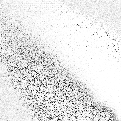
\includegraphics[width=\stratgraphwidthsmall]{images/findings/experiments/decay/decay_000_250.png}} & % 250
			\parbox[c]{5em}{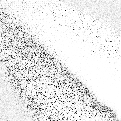
\includegraphics[width=\stratgraphwidthsmall]{images/findings/experiments/decay/decay_000_500.png}} & % 500
			\parbox[c]{5em}{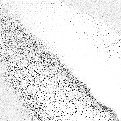
\includegraphics[width=\stratgraphwidthsmall]{images/findings/experiments/decay/decay_000_750.png}} & % 750
			\parbox[c]{5em}{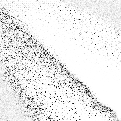
\includegraphics[width=\stratgraphwidthsmall]{images/findings/experiments/decay/decay_000_1mm.png}} \\ % 1mm
		\\
		0.10 & 
			\parbox[c]{5em}{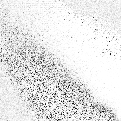
\includegraphics[width=\stratgraphwidthsmall]{images/findings/experiments/decay/decay_010_250.png}} & % 250
			\parbox[c]{5em}{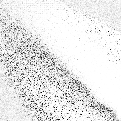
\includegraphics[width=\stratgraphwidthsmall]{images/findings/experiments/decay/decay_010_500.png}} & % 500
			\parbox[c]{5em}{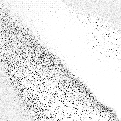
\includegraphics[width=\stratgraphwidthsmall]{images/findings/experiments/decay/decay_010_750.png}} & % 750
			\parbox[c]{5em}{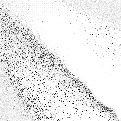
\includegraphics[width=\stratgraphwidthsmall]{images/findings/experiments/decay/decay_010_1mm.png}} \\ % 1mm
		\\
		0.25 & 
			\parbox[c]{5em}{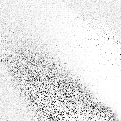
\includegraphics[width=\stratgraphwidthsmall]{images/findings/experiments/decay/decay_025_250.png}} & % 250
			\parbox[c]{5em}{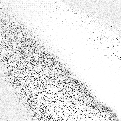
\includegraphics[width=\stratgraphwidthsmall]{images/findings/experiments/decay/decay_025_500.png}} & % 500
			\parbox[c]{5em}{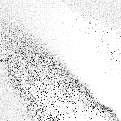
\includegraphics[width=\stratgraphwidthsmall]{images/findings/experiments/decay/decay_025_750.png}} & % 750
			\parbox[c]{5em}{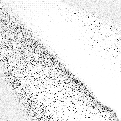
\includegraphics[width=\stratgraphwidthsmall]{images/findings/experiments/decay/decay_025_1mm.png}} \\ % 1mm
		\\
		0.50 & 
			\parbox[c]{5em}{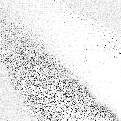
\includegraphics[width=\stratgraphwidthsmall]{images/findings/experiments/decay/decay_050_250.png}} & % 250
			\parbox[c]{5em}{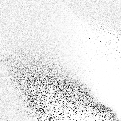
\includegraphics[width=\stratgraphwidthsmall]{images/findings/experiments/decay/decay_050_500.png}} & % 500
			\parbox[c]{5em}{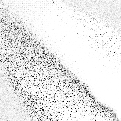
\includegraphics[width=\stratgraphwidthsmall]{images/findings/experiments/decay/decay_050_750.png}} & % 750
			\parbox[c]{5em}{
\includegraphics[width=\stratgraphwidthsmall]{images/findings/experiments/decay/decay_050_1mm.png}} \\ % 1mm
	\end{tabular}

\caption{
	Comparison of different decay rates learning the \handmaxavg\ strategy
	when playing as the dealer
	over the course of one million games.
	}
\label{fig:expts-decay-comp}
\end{figure}


